\documentclass[]{article}
\usepackage[a4paper, total={15cm,23cm}]{geometry}
\usepackage{fancyhdr}
\usepackage{graphicx}
\usepackage{amsmath}
\usepackage{amssymb}
\usepackage{xcolor}
\usepackage{tikz}
\usepackage{verbatim}
\usepackage{tcolorbox}
\usepackage{textcomp}
\usepackage{xcomment}
\usepackage{xstring}
\usepackage{array}
%opening
\title{Two Vector Hike}
\author{Benjamin Bauml}
\date{Spring 2024}
\pagestyle{fancy}
\rhead{PH 221}
\chead{Spring 2024}
\lhead{Week 1}

% Version 2024-02-21
% Changes
% 2024-02-21 Added xstring package to enable smooth implementation of new \ModePage command.
% For Assignment, leave Purpose as 1. For Worksheet, set to 2. For Student Solution, set to 3. For Teacher Solution, set to 4.
\newcommand{\Purpose}{4}

\newcommand{\Exclusion}{0}
\newcommand{\PageTurn}{0}
\newcommand{\GrayProb}{0}
\newcommand{\Tipsy}{0}

% Assignment
\if\Purpose1
\renewcommand{\Exclusion}{1}
\fi
% Worksheet
\if\Purpose2
\renewcommand{\Exclusion}{1}
\renewcommand{\PageTurn}{1}
\fi
% Student Solution
\if\Purpose3
\renewcommand{\PageTurn}{1}
\renewcommand{\GrayProb}{1}
\fi
% Teaching Copy
\if\Purpose4
\renewcommand{\PageTurn}{1}
\renewcommand{\GrayProb}{1}
\renewcommand{\Tipsy}{1}
\fi

\if\Exclusion1
\xcomment{Title,Problem,ProblemSub,PassFig}
\fi

\def \NewQ {0}
\def \PForce {0}
\newcommand{\MaybePage}[1]{
	\def \PForce {#1}
	\if\PForce1
		\newpage
	\else
		\if\NewQ0
		\gdef \NewQ {\PageTurn}
		\else
		\newpage
		\fi
	\fi
}

\newcommand{\ModePage}[1]{
	\IfSubStr{#1}{\Purpose}{\newpage}{}
}

\newenvironment{Problem}[2][0]{%The first argument is optional, and if it is set to 1, the \newpage will be forced.
\MaybePage{#1}
\section*{#2}
\if\GrayProb1
\begin{tcolorbox}[colback=lightgray,colframe=lightgray,sharp corners,boxsep=1pt,left=0pt,right=0pt,top=0pt,bottom=0pt,after skip=2pt]
\else
\begin{tcolorbox}[colback=white,colframe=white,sharp corners,boxsep=1pt,left=0pt,right=0pt,top=0pt,bottom=0pt,after skip=2pt]
\fi
}{
\end{tcolorbox}\noindent
}

\newenvironment{ProblemSub}[1][0]{%The argument is optional, and if a string of numbers is entered into it, it will force a \newpage in any \Purpose that shows up in the string. For example, "13" would lead to the newpage being forced in modes 1 and 3.
\ModePage{#1}
\if\GrayProb1
\begin{tcolorbox}[colback=lightgray,colframe=lightgray,sharp corners,boxsep=1pt,left=0pt,right=0pt,top=0pt,bottom=0pt,after skip=2pt]
\else
\begin{tcolorbox}[colback=white,colframe=white,sharp corners,boxsep=1pt,left=0pt,right=0pt,top=0pt,bottom=0pt,after skip=2pt]
\fi
}{
\end{tcolorbox}\noindent
}

\newenvironment{PassFig}{\begin{figure}[h]}{\end{figure}}

\newcommand{\TeachingTips}[1]{
\if\Tipsy1
\begin{tcolorbox}[colback=lightgray,colframe=black]
#1
\end{tcolorbox}
\fi
}

\newenvironment{Title}{\maketitle}{}

\begin{document}
\begin{Title}
\begin{center}
	This material is borrowed/adapted from PH 201 Tutorial 1 for Fall 2020.
\end{center}
\end{Title}

\begin{Problem}{Activity}
	Maria hikes 15.0 km at an angle of 30.0$ ^{\circ} $ north of east and then hikes 15.0 km southeast (an angle of 45.0$ ^{\circ} $ south of east). Let Maria's starting point be the origin of your coordinate system, the east-west axis be horizontal, and the north-south axis be vertical with east and north the positive directions.
\end{Problem}
\begin{ProblemSub}
	a) Draw a sketch, approximately to scale, showing the coordinate axes, Maria's two displacements, and her total displacement.
\end{ProblemSub}
\begin{figure}[h]
	\centering
	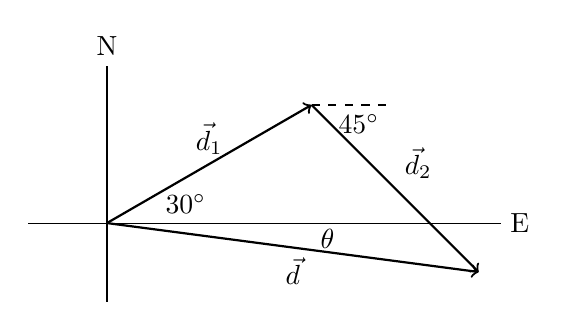
\begin{tikzpicture}
		\draw (0,-1) -- (0,2);
		\node[anchor=south] at (0,2) {N};
		\draw (-1,0) -- (5,0);
		\node[anchor=west] at (5,0) {E};
		\draw[->,thick] (0,0) -- ({3*cos(30)},{3*sin(30)});
		\node[anchor=south] at ({1.5*cos(30)},{1.5*sin(30)}) {$\vec{d}_{1}$};
		\node[anchor=south] at (1,0) {$30^{\circ}$};
		\draw[dashed] ({3*cos(30)},{3*sin(30)}) -- ({3*cos(30)+1},{3*sin(30)});
		\node[anchor=north] at ({3*cos(30)+0.6},{3*sin(30)}) {$45^{\circ}$};
		\draw[->,thick] ({3*cos(30)},{3*sin(30)}) -- ({3*cos(30)+3*cos(45)},{3*sin(30)-3*sin(45)});
		\node[anchor=south west] at ({3*cos(30)+1.5*cos(45)},{3*sin(30)-1.5*sin(45)}) {$\vec{d}_{2}$};
		\draw[->,thick] (0,0) -- ({3*cos(30)+3*cos(45)},{3*sin(30)-3*sin(45)});
		\node[anchor=north] at ({1.5*cos(30)+1.5*cos(45)},{1.5*sin(30)-1.5*sin(45)}) {$\vec{d}$};
		\node[anchor=north] at (2.8,0.05) {$\theta$};
	\end{tikzpicture}
\end{figure}

\noindent\textbf{Known:}
\begin{itemize}
	\item $ d_{1} = 15.0\text{ km};\ \theta_{1} = 30.0^{\circ} $
	\item $ d_{2} = 15.0\text{ km};\ \theta_{2} = -45.0^{\circ} $
\end{itemize}
\textbf{Find:} $ d,\ \theta $
\begin{ProblemSub}
	b) Find the east ($ x $) and north ($ y $) components of Maria's two displacements.
\end{ProblemSub}
\[
\begin{split}
	d_{1E} & = d_{1}\cos\theta_{1} = (15.0\text{ km})\cos30.0^{\circ} = 12.99\text{ km} \\
	d_{1N} & = d_{1}\sin\theta_{1} = (15.0\text{ km})\sin30.0^{\circ} = 7.50\text{ km} \\
	d_{2E} & = d_{2}\cos\theta_{2} = (15.0\text{ km})\cos(-45.0^{\circ}) = 10.61\text{ km} \\
	d_{2N} & = d_{2}\sin\theta_{2} = (15.0\text{ km})\sin(-45.0^{\circ}) = -10.61\text{ km} \\
\end{split}
\]
\begin{ProblemSub}
	c) Find the east ($ x $) and north ($ y $) components of Maria's total displacement.
\end{ProblemSub}
\[
\begin{split}
	d_{E} & = d_{1E} + d_{2E} = 12.99\text{ km} + 10.61\text{ km} = 23.60\text{ km} \\
	d_{N} & = d_{1N} + d_{2N} = 7.50\text{ km} + (-10.61\text{ km}) = -3.11\text{ km} \\
\end{split}
\]
\begin{ProblemSub}
	d) Find the magnitude and direction of Maria's total displacement.
\end{ProblemSub}
\[
\begin{split}
	d & = \sqrt{d_{E}^{2}+d_{N}^{2}} = \sqrt{(23.60\text{ km})^{2} + (-3.11\text{ km})^{2}} = 23.8\text{ km} \\
	\theta & = \tan^{-1}\left(\frac{d_{N}}{d_{E}}\right) = \tan^{-1}\left(\frac{-3.11\text{ km}}{23.60\text{ km}}\right) = -7.50^{\circ}
\end{split}
\]
\begin{ProblemSub}
	e) Check your answer to (d) against your sketch. Do they agree?
\end{ProblemSub}
Maria's displacement was 23.8 km at an angle of 7.50$ ^{\circ} $ south of east. This agrees with the sketch which shows a small angle below the x-axis. Note that the magnitude of her total displacement is only slightly greater than her total horizontal displacement because the angle is small.

In adding vectors by components, it is important to keep track of their signs. If we hadn’t had the negative sign in the north component of Maria’s second hike, our answer would have been much different (and wrong).
\end{document}